
\chapter{A Problem of Composition}

Pattern matching is a useful technique when manipulating data. This
chapter describes how to implement pattern directed rules that transform
data and how to address a problem that arises with this approach.
The implementation also shows how to use operations to delay expressions
in rules and how to get the variables bound by the pattern matching
into the delayed expressions.

When mapping models to code (and other structured targets) it would
be nice of the structure of the target matched the structure of the
source. When this happens, individual elements in the source model
can be transformed into elements of the target model, and the resulting
target elements are then just grouped together to form the result.
For example, when translating UML model classes with attributes to
Java class definitions, each UML class turns into a Java class definition,
each attribute in the UML class produces a corresponding attribute
in the Java class. The structure is the same, but the detail of representation
is different.

Unfortunately this situation does not often occur. For example, UML
models consist of separate elements for classes, associations and
state machines; each of these model elements are distinct, but they
reference each other. A translation from UML to Java may choose to
produce a single class definition consisting of:

\begin{itemize}
\item Java classes for UML classes;
\item Java fields for UML class attributes and association role ends;
\item A state field.
\item An enumeration in each Java class for each UML message.
\item A single Java method in a class for handling messages;
\item A case for each transition within the message handler.
\end{itemize}
The information in the Java program is nested within the Java class.
The corresponding information in the UML model is spread out. The
structures are not equivalent.

It is certainly possible to pass tables around the source model and
build up the required parts of the target model. However, it is possible
to do better than that and to use a language driven approach to hide
away the details of how the target model is built up. The transformation
language constructs can be pattern directed and the output can be
declarative in such a way as to focus on mapping source elements to
target elements without having to say too much about the mechanisms
by which the output is produced.

This chapter is about the design of a language for producing code
for models that solves the composition problem. The structure of this
chapter is as follows: section \ref{sec:Translating-Executable-Models}
describes a simple executable model and its translation to Java; section
\ref{sec:Transformation-Architecture} describes the architecture
of the solution; section \ref{sec:A-Rule-Based-Language} describes
a language for rule based model transformation and shows how it can
be used to implement the transformation rules for the example; section
\ref{sec:Rules-Implementation} provides the implementation of the
language constructs.


\section{Translating Executable Models\label{sec:Translating-Executable-Models}}

This section describes a typical scenario where the translation from
models to program code requires the target code to pull together information
from different parts of the source model. A fully executable program
is produced by translating class models and state machines to Java.
The example is a car cruise controller and is very simple, but is
representative of a large number of strategies for producing programs
from models.

%
\begin{figure}
\begin{center}

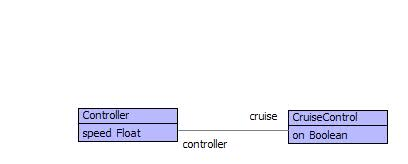
\includegraphics[width=12cm]{LanguageEngineering/DocComposition/Images/Controller}

\caption{Classes for a simple cruise control in a car engine system. Typical
of a system that is to be controlled via a state machine.\label{fig:Cruise-Control-Model}}

\end{center}
\end{figure}


Figure \ref{fig:Cruise-Control-Model} shows a simple model consisting
of classes, attributes and associations. A car engine controller manages
the speed of the car and communicates with the cruise control system.
The cruise control system is managed via a mechanical switch on the
dashboard.

%
\begin{figure}
\begin{center}

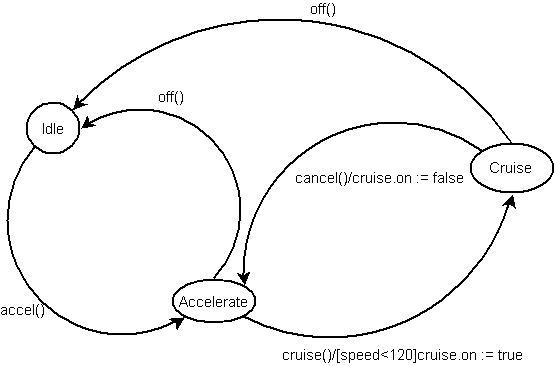
\includegraphics[width=12cm]{LanguageEngineering/DocComposition/Images/Accel}

\caption{A state machine describing the behaviour of the Controller class for
the car cruise control system. The controller exists in one of the
states (labelled ellipses). Transitions between states occur when
the controller receives the messages. Guards in {[} and ] determine
whether the transition is legal. Actions on the transitions describe
what happens when the transition takes place.\label{fig:Cruise Control}}

\end{center}
\end{figure}


Figure \ref{fig:Cruise Control} shows a state machine that defines
the behaviour of the engine controller. The engine starts in the Idle
state when it is switched on. When the controller detects the accelerator
being pressed, it switches to the Accelerate state. When the car is
accelerating, the driver can press the cruise control button on the
dashboard causing the controller to switch to the Cruise state providing
that the speed is less than a preset amount (120). In the cruising
state, the driver can switch the control off by pressing the accelerator.
When switching to and from the cruising state, the engine controller
communicates with the cruise controller, setting its 'on' state.

Given the behavioural models defined in figures \ref{fig:Cruise-Control-Model}
and \ref{fig:Cruise Control}, it is possible to produce a fully executable
Java program. The program consists of class definitions for the two
classes in the model. Each class includes fields, accessors, updaters
and a message handling operation; the definition of these components
comes from different aspects of the source model. 

The rest of this section shows the program code generated from the
Controller class. The example is representative of the code generated
from any class in a behavioural model. Firstly, each model class produces
a Java class definition (the missing definitions are given subsequently):

\begin{lstlisting}
class Controller {
  // Messages...
  // Fields...
  // Accessors...
  // Updaters...
  // Message passing...
}
\end{lstlisting}The state machine for a class defines a collection of messages on
the transitions. Each of the messages has a unique identifier that
is defined as a collection of constants in the class:

\begin{lstlisting}
  // Messages...
  public static final int accel  = 0;
  public static final int cruise = 1;
  public static final int off    = 2;
  public static final int cancel = 3;
\end{lstlisting}The state of an object is given by field definitions that come from
different aspects of the behavioural model:

\begin{itemize}
\item Each model class defines a collection of attributes with simple types
(such as String or Integer); for example the engine controller class
defines an attribute 'speed' of type 'Float'. 
\item The model requires that each object exists in one of a given number
of states; for example the engine controller has states for Idle,
Cruise and Accelerate.
\item The model contains a number of associations between classes. The associations
allow instances of the classes to communicate with each other. The
engine controller class has an association with the cruise controller
class with role end names cruise and controller.
\end{itemize}
The Java field definitions for the engine controller are given below:

\begin{lstlisting}
  // Fields...
  Float speed;          // Simple attribute.
  String state;         // Current state.
  CruiseControl cruise; // Association role end.
\end{lstlisting}Each of the Java fields given above are private to the class definition.
To provide access to the state of a Java instance, the following accessors
and updaters are defined:

\begin{lstlisting}
  // Accessors and updaters...
  public CruiseControl getcruise() { return cruise; }
  public Float getspeed() { return speed; }
  public void setcruise(CruiseControl cruise) { 
    this.cruise = cruise; 
  }
  public void setspeed(Float speed) { 
    this.speed = speed; 
  }
\end{lstlisting}State machines define the behaviour of objects in response to receiving
messages. This can be defined in Java using a method in each class
that handles messages:

\begin{lstlisting}
public void send(int message,Object[] args) {
  switch(message) {
    // Transitions...
  }
}
\end{lstlisting}Each transition consists of source and target states s and t, the
transition occurs when a message m is received and when a guard g
is true. When the transition fires, an action a is performed and the
receiver changes to the target state t. Each message is implemented
as a case in the Java switch statement:

\begin{lstlisting}
    case m:
      // Transition...
      if(state == s && g) {
        a;
        state = t;
      }
      break;
\end{lstlisting}
The state machine for the engine controller is shown below:

\begin{lstlisting}
  // Message passing...
  public void send(int message,Object[] args) {
    switch(message) {
      case Controller.accel:
        if(state.equals("Idle"))
          state = "Accelerate";
        break;
      case Controller.cruise:
        if(state.equals("Accelerate") && speed < 120)
          cruise.seton(true);
          state = "Cruise";
        break;
      case Controller.off:
        if(state.equals("Accelerate"))
          state = "Idle";
        break;
      case Controller.cancel:
        if(state.equals("Cruise"))
          cruise.seton(false);
          state = "Accelerate";
        break;
      case Controller.off:
        if(state.equals("Cruise"))
          state = "Idle";
        break;
      default: throw new Error("No message " + message);
    }
\end{lstlisting}
\section{Transformation Architecture\label{sec:Transformation-Architecture}}

Before looking at a language that supports the generation of code
for models, it is worth considering the steps taken by a mechanical
process. The idea is that the mechanical process is driven by code
generation rules and that the rules encode any domain specific information
about the models being transformed. The code generation rules are
pattern directed and follow the structure of the source model:

\begin{lstlisting}
for each class c
  emit a Java class definition.
  emit a state field.
  for each attribute a of c
    emit a field definition for a.
    emit an access and updater for a.
  emit a message handling method.
for each association A
  emit a field for end1
  emit a field for end2
for each state machine m for class c
  for each transition t of m
    emit a constant field to c for message(t)
    emit a message case for t to c
\end{lstlisting}The transformation defined above follows the structure of the source
model. However, the code that is produced (or \emph{emitted}) by the
transformation rules does not follow the same structure; for example
fields arising from associations must be added to class definitions
that are produced by other parts of the transformation. It is attractive
to have the transformation follow the structure of the source model
but some technology must be employed to tie up the various target
components. An effective way to do this is to use labels: emitted
code is labelled and may contain labels, once the labelled target
components are produced a subsequent phase is used to resolve label
references.

%
\begin{figure}
\begin{center}

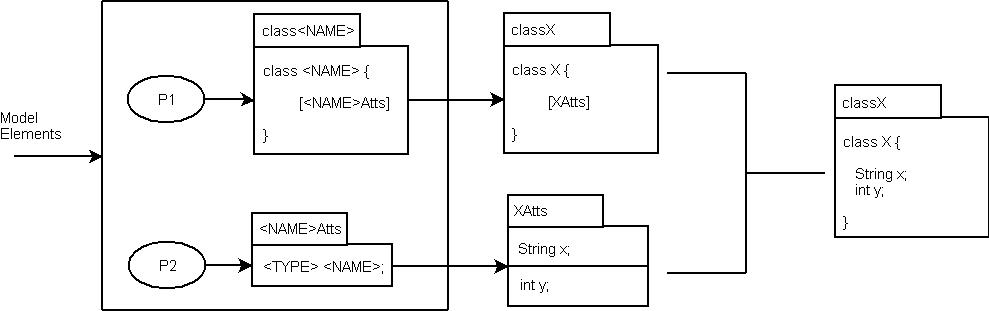
\includegraphics[width=12cm]{LanguageEngineering/DocComposition/Images/Templates}

\caption{An overview of rule firing. Elements match against patterns, document
templates are produced. The templates contain label references. A
resolution step replaces label references with the documents that
they refer to.\label{fig:Mapping-Cycle}}

\end{center}
\end{figure}


An overview of the architecture of the transformation process shown
in figure \ref{fig:Mapping-Cycle}. Model elements are supplied to
the rules in the rule base. Each rule consists of a source pattern
and a target pattern. Two rules are shown:

\begin{enumerate}
\item R1: Pattern P1 matches a class in the model. The output pattern describes
a Java class labelled with the class name.
\item R2: Pattern P2 matches an attribute in the model. The output pattern
describes a Java field labelled with the name of the owning class.
\end{enumerate}
When model elements are supplied to a rule-base consisting of a collection
of rules, each rule is tried in turn. If the input elements match
the patterns then the rule is \emph{enabled}. Patterns contain variable
names and an enabled rule has an \emph{environment} of variable bindings.
The first enabled rule is \emph{fired}. Firing a rule produces a \emph{document
template} by replacing all occurrences of pattern variables in the
output pattern. Turning an output pattern into a document template
is referred to as \emph{forcing} the output pattern with respect to
the environment. 

Figure \ref{fig:Mapping-Cycle} shows three document templates produced
from the rule-base. The first is labelled with classX and is the result
of mapping a model class named X to a Java class. The second and third
are both labelled with XAtts and are the result of mapping two class
attributes named x and y to Java fields. The classX template contains
a reference to a label XAtts that is a placeholder for the fields
of the class. 

A document template is transformed into a document by replacing all
label references with documents. This process is called \emph{displaying}
the document template. The display process is shown as the final step
in figure \ref{fig:Mapping-Cycle} where the occurrence of XAtts in
the class definition is replaced with all the field definitions labelled
XAtts.

Rule firing may involve multiple passes over the data; the output
pattern of each rule may refer to other rule-bases (including its
own) and supply data to those rule-bases to produce the final document
templates. For example, the rule R1 is supplied with a class, emits
a document template for the class but also calls the rule-base again
with the attributes of the class so that rule R2 fires on each attribute.
All rule firing is completed before document display takes place.


\section{A Rule Based Language\label{sec:A-Rule-Based-Language}}

The transformation from a model to code is performed by a rule-base
containing a collection of rules. The rule base is supplied with one
or more model elements as input. It tries the rules in turn until
one of the rules matches the input. The body of the matching rule
is forced to produce a document template. The template may be labelled
and may contain labelled placeholders. The rule-base may be performed
multiple times against different model elements. Once execution is
complete, the templates are displayed by matching placeholder labels
against labelled output. The result is an output document with no
unresolved labels that can be displayed as text. This section describes
the features of the rule-base language and concludes with the complete
behavioural modelling rule-base as described in the previous section.

A rule-base with the name N has the following format:

\begin{lstlisting}
@RuleBase N
  // Rules...
end
\end{lstlisting}A rule named R has the following format:

\begin{lstlisting}
@Rule R P1,P2,...,Pn -> 
  D1 D2 ... Dm 
end
\end{lstlisting}where each Pi is an element pattern and each Di is a document pattern.
The idea of a rule is that it must be supplied with n inputs. If each
of the n inputs match the patterns then the rule is \emph{enabled}.
An enabled rule is \emph{fired} by forcing the output defined by each
Di in turn. The result produced by the rule firing is the last document
Dm. Each pattern Pi may contain variables that match against the corresponding
input. If the rule is enabled then the collection of variables and
values provides an environment for the rule firing.

Here is a simple example of a rule:

\begin{lstlisting}
@Rule Anything x ->
  <x>
end
\end{lstlisting}The pattern 'x' matches anything as input. A document < exp > performs
the expression exp in the supplied rule-firing environment. The result
of x is either a document or an element that is transformed into a
string. In the case of Anything, the rule will produce the stringified
version of x as a document.

A pattern may match an object:

\begin{lstlisting}
@Rule ToJava Class[name=n] ->
  "public class " + <n> + "{"
end
\end{lstlisting}The pattern in the rule ToJava matches instances of Class and matches
the name of the class with the variable 'n'. Two documents are composed
using the '+' operator. Supplying the class Element to this rule (firing
and displaying the result) produces:

\begin{lstlisting}
public class Element {
\end{lstlisting}Indentation in a document is produced using the matching directives
->{[} and ]:

\begin{lstlisting}
@Rule ToJava Class[name=n] ->
  "public class " + <n> + "{" +
    ->[ nl +
        "public String state;"
    ] + nl +
   "}"
end
\end{lstlisting}Supplying Element to the above rule produces:

\begin{lstlisting}
public class Element {
  public String state;
}
\end{lstlisting}The nl directive produces a newline and tabs to the current level
of indentation. Collections are processed using the \{ and \} directives:

\begin{lstlisting}
@Rule ToJava Class[name=n,attributes=A] ->
  "public class " + <n> + "{" +
    ->[ nl +
        "public String state;" + nl
        { <A> <map> nl empty }
    ] + nl +
  "}"
end
\end{lstlisting}The \{ and \} contain four components \{ S M C D \} where: S defines
the collection; M defines a mapping that is applied to each element
of S in turn; C is a document combinator and D is a default document.
The easiest way to understand this construct is via an example. Given
a collection S = \{x,y,z\} then \{ S M C D\} produces C(M(x),C(M(y),M(z))).
Given a collection S = \{\} then the default D is produced.

The collection component S may be a label or an expression. In the
example above <A> is an expression where A is provided by the context
of the rule firing. The mapping component M is an expression. The
variable map always refers to the containing rule-base and therefore
allows the rule base to be applied as part of a rule firing. The combiner
nl causes the documents to be combined by joining them together with
newlines. The document empty is just that. Note that nl and empty
are builtin so we don't put < and > round them.

Suppose that C is a class with two attributes x and y of type String
and Integer respectively. Using the above definition to transform
C produces the following (assuming suitable rule definitions for attribute
to field transformation):

\begin{lstlisting}
public class C {
  public String state;
  String x;
  int y;
}
\end{lstlisting}The ToJava rule above is incomplete since there is no rule for mapping
attributes, here they are:

\begin{lstlisting}
@Rule MapStrAtt 
  Attribute[name=n,type=NamedElement[name="String"]] -> 
    "String " + <n> + ";" 
end
@Rule MapIntAtt 
  Attribute[name=n,type=NamedElement[name="Integer"]] -> 
    "int " + <n> + ";" 
end
// More cases...
\end{lstlisting}Labels can be used either by themselves in documents or as the source
of collection templates (as in <A> above). Documents can be tagged
with labels using 'emit'. Here are the class and attribute rules re-written
to use labels:

\begin{lstlisting}
@Rule ToJava Class[name=n,attributes=A] ->
  "public class " + <n> + "{" +
    ->[ nl +
        "public String state;" + nl
        { [n + "Atts"] <@Operation(a) map(a,n) end> nl empty }
    ] + nl +
  "}"
end
@Rule MapStrAtt 
  Attribute[name=n,type=NamedElement[name="String"]],
  className -> 
    emit[className + "Atts"]
      "String " + <n> + ";" 
end
\end{lstlisting}Notice that the mapping components of the collection expression is
modified to become an operation that supplies two elements to the
mapping (a,n). Each attribute mapping rule has two inputs: the attribute
and the name of the class. The attribute rule emits (and returns)
a Java field definition. When a document is emitted against a label
(in this case className + {}``Atts''), it is added to the collection
of documents for that label. When the resolution phase is performed,
the collection expression will use all of the documents registered
against the label.

This concludes the overview of the rule language for transforming
model elements. The key features of element patterns are: constants;
variables; object patterns with slots. The key features of the document
patterns are: literal strings; delayed expressions in < ... >; combination
with +; indentation and newlines with ->{[} ... ] and nl; labels with
{[} ... ]; tagged documents using 'emit'; combining collections with
\{ ...\}.

Finally, the rules for the Java mapping are defined below. There are
two rule bases. The first is used to map model types to Java types
and the second is used to map packages, classes, attributes and state
machines to Java classes. The first rule base is defined in its entirety
below and the second is defined on a rule-by-rule basis.

Model types are named elements. The names must be mapped to the appropriate
Java types. To simplify the example, sets and sequences are translated
to vectors:

\begin{lstlisting}
@RuleBase Types
  @Rule String NamedElement[name='String'] ->
    "String"
  end
  @Rule Integer NamedElement[name='Integer'] ->
    "int"
  end
  @Rule Integer NamedElement[name='Boolean'] ->
    "boolean"
  end
  @Rule Sequence Seq[elementType=t] ->
    "Vector<" + <map(t)> + ">"
  end
  @Rule Set Set[elementType=t] ->
    "Vector<" + <map(t)> + ">"
  end
  @Rule Default NamedElement[name=n] -> 
    <n>
  end
\end{lstlisting}A package is a collection of classes, associations and sub-packages.
Each package gives rise to a document labelled with the name of the
package. The contents of the document are produced by mapping the
contents:

\begin{lstlisting}
@Rule TranslatePackage 
  Package[name=n,classes=C,associations=A,packages=P] ->
    emit["Package-" + n] 
      { <C> <map> nl empty } +
      { <A> <map> nl empty } +
      { <P> <map> nl empty }
end
\end{lstlisting}A class is transformed into a Java class definition. Some of the components
of the Java class can be produced directly from the model, other components
are produced from model elements that originate elsewhere. The following
rule uses labels as placeholders for the program code that is generated
elsewhere. The comments in the rule describe each of the major components:

\begin{lstlisting}
@Rule TranslateClass 
 Class[name=n,attributes=A] ->
  // Emit a labelled class definition...
  emit["Class-" + n]
   "class " + <n> + " {" + 
   // Indent the body of the definition...
   ->[ nl +
     // Transitions define messages, 
     // each message defines a constant...
     { [n + "transitions"] id nl empty } + nl +
     // Each attribute defines a simple-typed Java field...
     { <A> < @Operation(a) map(a,n) end> nl empty } + nl +
     // Each instance has its own state...
     "String state;" + nl +
     // Attributes are defined by associations...
     { [n + "attributes"] id nl empty } + nl +
     // Accessors and updaters are defined elsewhere...
     { [n + "accessors"] id nl empty } + nl +
     { [n + "updaters"] id nl empty } + nl +
     // Each class has a message handler...
     "public void send(int message,Object[] args) {" +
     // Indent the body of the method...
     ->[ nl + 
       "switch(message) {" +
       // Indent the body of the switch
       ->[ nl +
         // Each transition produces a message case...
         { [n + "messages"] id nl empty } + nl +
         // In case the message is not handled...
         "default: throw new Error(\"No message \" + message);" 
       ] + nl + 
       "}"
     ]
   ] + nl +
  "}"
end
\end{lstlisting}Each attribute defined by a class in the model produces an accessor,
an updater and a Java field definition. The methods are labelled so
that all accessors and updaters for the class are defined in the same
place in the output. The field definition is returned:

\begin{lstlisting}
@Rule TranslateAttribute Attribute[name=n,type=t],c ->
  // Produce an accessor method for this field...
  emit[c + "accessors"]
    <Types.apply(t)> + " get" + <n> + "()" +
    "{ return " + <n> + "; }"
  // Produce an updater method for this field...
  emit[c + "updaters"]
    "void set" + <n> + "(" + <Types.apply(t)> + " " + <n> + ")" +
    "{ this." + <n> + " = " + <n> + "; }"
  // Produce the field definition...
  <Types.apply(t)> + " " + <n> + ";"
end
\end{lstlisting}An association consists of two ends; each end has a name and is attached
to a type. An association produces a pair of field definitions in
the Java classes and also adds accessors and updaters. The transformation
is performed by the following two rules:

\begin{lstlisting}
@Rule TranslateAssociation Association[end1=e1,end2=e2] ->
  // Produce definitions for the class at end1...
  <map(e1,e2)>
  // Produce definitions for the class at end2...
  <map(e2,e1)>
  // Just for side effect...
  empty
end

@Rule TranslateEnd 
  End[name=n1,type=t1],End[name=n2,type=t2] ->
  // produce a field definition for the class t1...
  emit[t1.name() + "attributes"]
    <Types.apply(t2)> + " " + <n2> + ";"
  // Produce an accessor method for t1...
  emit[t1.name() + "accessors"]
    "public " + <Types.apply(t2)> + " get" + <n2> + "() { " +
    ->[ nl + 
      "return " + <n2> + ";" + nl  
    ] + nl + "}"
  // produce an updater for t1...
  emit[t1.name() + "updaters"]
    "public void set" + <n2> + 
      "(" + <Types.apply(t2)> + " " + <n2> + ") { " +
    ->[ nl + 
      "this." + <n2> + " = " + <n2> + ";" + nl  
    ] + nl + "}"
end
\end{lstlisting}A state machine belongs to a class and defines states and transitions.
The state machine is implemented in Java as an enumerated type for
the messages and as a message handling method. Each transition defines
what happens when an instance of the class receives a message. A message
is defined as an enumerated type implemented as a bunch of constants
in the class. A transition is implemented as a case in the message
handling method. The rest of the rules define the transformation of
a state machine to its implementation.

\begin{lstlisting}
@Rule TranslateMachine StateMachine[class=c,states=S,trans=T] ->
  // Translate the messages to constants. Use ->asSet
  // to remove duplicate message names...
  <map(T.message->asSet->asSeq,T.message->asSet->asSeq,c)>
  // translate the transitions to message handling cases...
  <map(T,c)>
end
\end{lstlisting}The following rules produce constant definitions for the messages
used by the state machine:

\begin{lstlisting}
@Rule TranslateMessages allMessages,Seq{message|messages},class ->
  // Produce a constant (use the position 
  // of the name as its value)...
  <map(message,class,allMessages->indexOf(message))>
  // Map the rest of the messages...
  <map(allMessages,messages,class)>
end
@Rule NoMessagesLeft allMessages,Seq{},class ->
  // No messages, requires no constants...
  empty
end
@Rule TranslateMessage message,Class[name=className],index ->
  // Produce a constant with value index...
  emit[className + "transitions"]
    "public static int " + <message> + " = " + <index> + ";"
end
\end{lstlisting}Finally, each transition produces a case entry in the message handling
method of the class. The case checks that the receiver is in the correct
state and that the guard is true. If so then the action is performed
and the receiver changes to the target state:

\begin{lstlisting}
@Rule TranslateTrans Seq{
  Trans[source=s,        // Source state name
        target=t,        // Target state name
        message=m,       // Message name
        condition=p,     // Condition (Java code)
        action=a         // Action (Java code)
       ] | T},           // T is more transitions
  c ->                   // Class that owns the transition
  // Produce a case definition for the message handling
  // method for class c...
  emit[c.name() + "messages"]
   // This case handles the message m...
   "case " + <c.name()> + "." + <m> + ":" + 
   ->[ nl + 
     // check we are in the appropriate state s and
     // the predicate p is true...
     "if(state.equals(" + <str(s)> + ") && " + <p> + ")" + 
     ->[ nl +
       // Perform the action...
       <a> + ";" + nl +
       // Change to the target state...
       "state = " + <str(t)> + ";"
     // Break out of the switch...
     ] + nl + "break;"
   ]
  // Translate the rest of the transitions...
  <map(T,c)>
end

@Rule TranslateNoTrans Seq{},c ->
  // The base case...
  empty
end
\end{lstlisting}
\section{Implementation\label{sec:Rules-Implementation}}

The previous section has defined the syntax of a language for pattern
directed document generation rules. The language addresses the code
generation composition problem whereby the structure of the input
model elements does not match the structure of the output code. Labels
are used to tag the generated code (or \emph{document} \emph{templates})
and to define placeholders that are then resolved in a subsequent
phase. 

This section defines the rule-based document generation language.
There are several parts to the definition: the language of patterns,
the language of documents and the label resolution mechanism. Each
of these are explained in turn.


\subsection{Pattern Matching}

%
\begin{figure}
\begin{center}

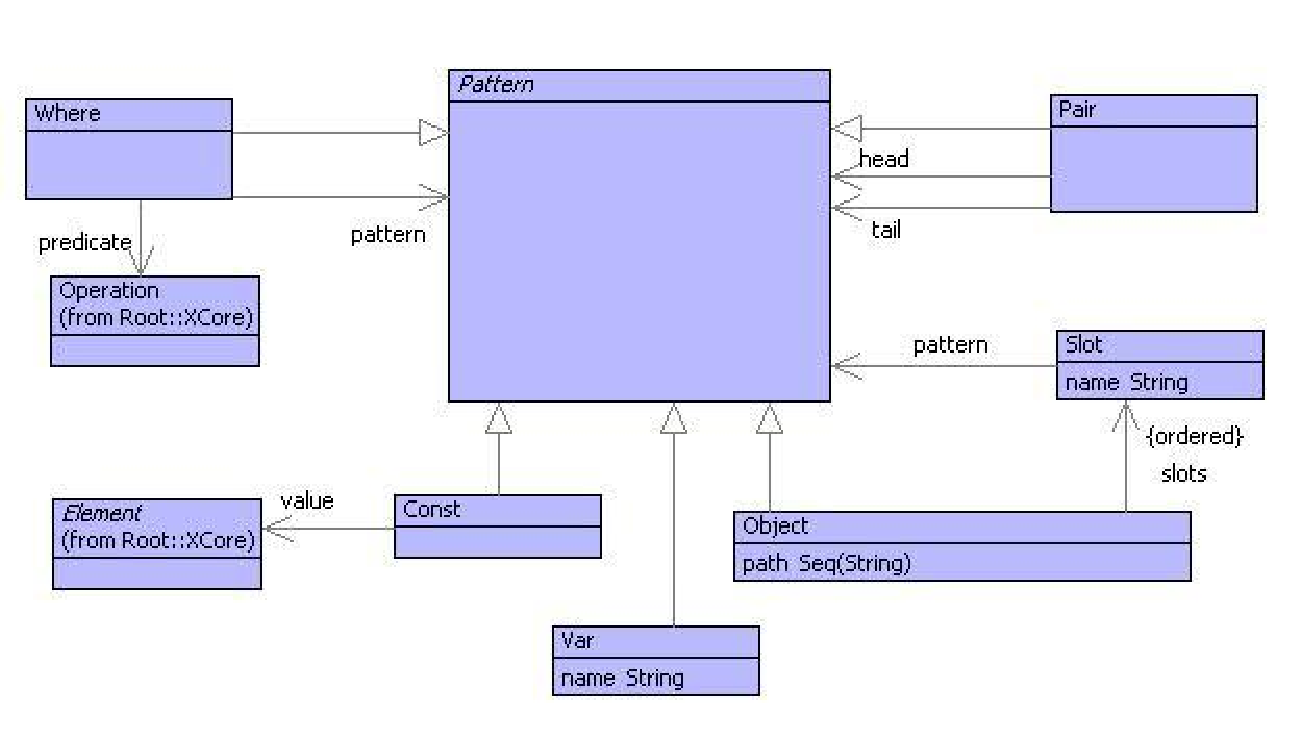
\includegraphics[width=12cm]{LanguageEngineering/DocComposition/Images/Pattern}

\caption{Patterns\label{fig:Patterns}}

\end{center}
\end{figure}


Figure \ref{fig:Patterns} shows the definition of a pattern language.
Patterns occur frequently in language definitions where it is useful
to extract elements from data depending on the structure of the data.
When this is a requirement is it almost always cost effective to define
a pattern language and a pattern matching mechanism that it is to
write the corresponding program code that extracts the elements each
time they are required. For example, the pattern:

\begin{lstlisting}
  C[x=10,y=v]
\end{lstlisting}is equivalent to the code:

\begin{lstlisting}
if element.isKindOf(C)
then
  if element.x = 10
  then // bind "v" to 10
  else // fail match
  end
else // fail match
end
\end{lstlisting}Given that patterns can involve multiple elements and can be nested,
the saving in terms of code is quite significant. Furthermore, modelling
the pattern language provides other benefits. The language becomes
circumscribed and its processing can be very effectively controlled.
For example error handling can be reported in terms of the original
patterns and not the implementation of the patterns. Optimizations
for pattern matching can be universally and retrospectively applied.
The patterns can be translated to other implementation platforms,
for example by exporting to a programming language.

The simplified grammar for patterns is shown below:

\begin{lstlisting}
@Grammar
  Constant ::= 
    s = Str { Const(s) } 
  | i = Int { Const(i) }  
  | 'true' { Const(true) } 
  | 'false' { Const(false) }.
  EmptySeq ::= '}' { Const(Seq{}) }.
  HeadTail ::= h = Pattern '|' t = Pattern '}' { Pair(h,t) }.
  Pair ::= 'Seq{' (HeadTail | EmptySeq).
  Path ::= p = ('::' Name)* { p }.
  Pattern ::= 
    Constant 
  | n = Name NameTail^(n) 
  | Pair.
  NameTail(n) ::= 
    p = Path '[' s = Slots ']' { Object(Seq{n|p},s) } 
  | { Var(n) }.
  Slots ::= 
    s = Slot ss = (',' Slot)* { Seq{s | ss} } 
  | { Seq{} }.
  Slot ::= n = Name '=' p = Pattern { Slot(n,p) }.
end 
\end{lstlisting}Given an element and a pattern, matching is implemented as a mechanism
that constructs an environment of variable bindings. Each binding
associates a variable with a value such that substituting each variable
for its value in the pattern produces the original element. For example,
given the pattern:

\begin{lstlisting}
  C[x=10,y=v]
\end{lstlisting}and an instance o of C such that o.x = 10 and o.y = 20 then the environment
associating y with 20 allows the pattern to be equivalent to the element
o. The mechanism is implemented by defining a match operation for
each of the pattern classes. Each operation is called match and expects
two arguments: the value to be matched and the current variable binding
environment. The result of the match is either the variable binding
environment or null, if the match fails. For constants:

\begin{lstlisting}
context Const
  @Operation match(value,env)
    if value = self.value
    then env
    else null
    end
  end
\end{lstlisting}A variable pattern matches anything:

\begin{lstlisting}
context Var
  @Operation match(value,env)
    env->bind(name,value)
  end
\end{lstlisting}A pair pattern must match a sequence (and not an empty sequence since
that is treated as a constant) such that the head and tail of the
pattern matches the corresponding elements of the value:

\begin{lstlisting}
context Pair
  @Operation match(value,env)
    if value.isReallyKindOf(Seq(Element)) and 
       not value = Seq{}
    then 
      env := head.match(value->head,env);
      if env <> null
      then tail.match(value->tail,env)
      else env
      end
    else null
    end
  end
\end{lstlisting}An object pattern matches an instance of the appropriate class where
all the slot patterns match the appropriate slot values:

\begin{lstlisting}
context Object
  @Operation match(value,env)
    if value.isReallyKindOf(self.classifier())
    then 
      @For slot in slots do
        if env <> null
        then env := slot.match(value,env)
        end
      end;
      env
    else null
    end
  end
\end{lstlisting}Each slot matches the appropriate slot value:

\begin{lstlisting}
context Slot
  @Operation match(object,env)
    if object.hasSlot(name)
    then pattern.match(object.get(name),env)
    else null
    end
  end
\end{lstlisting}
\subsection{Documents}

\begin{figure}
\begin{center}

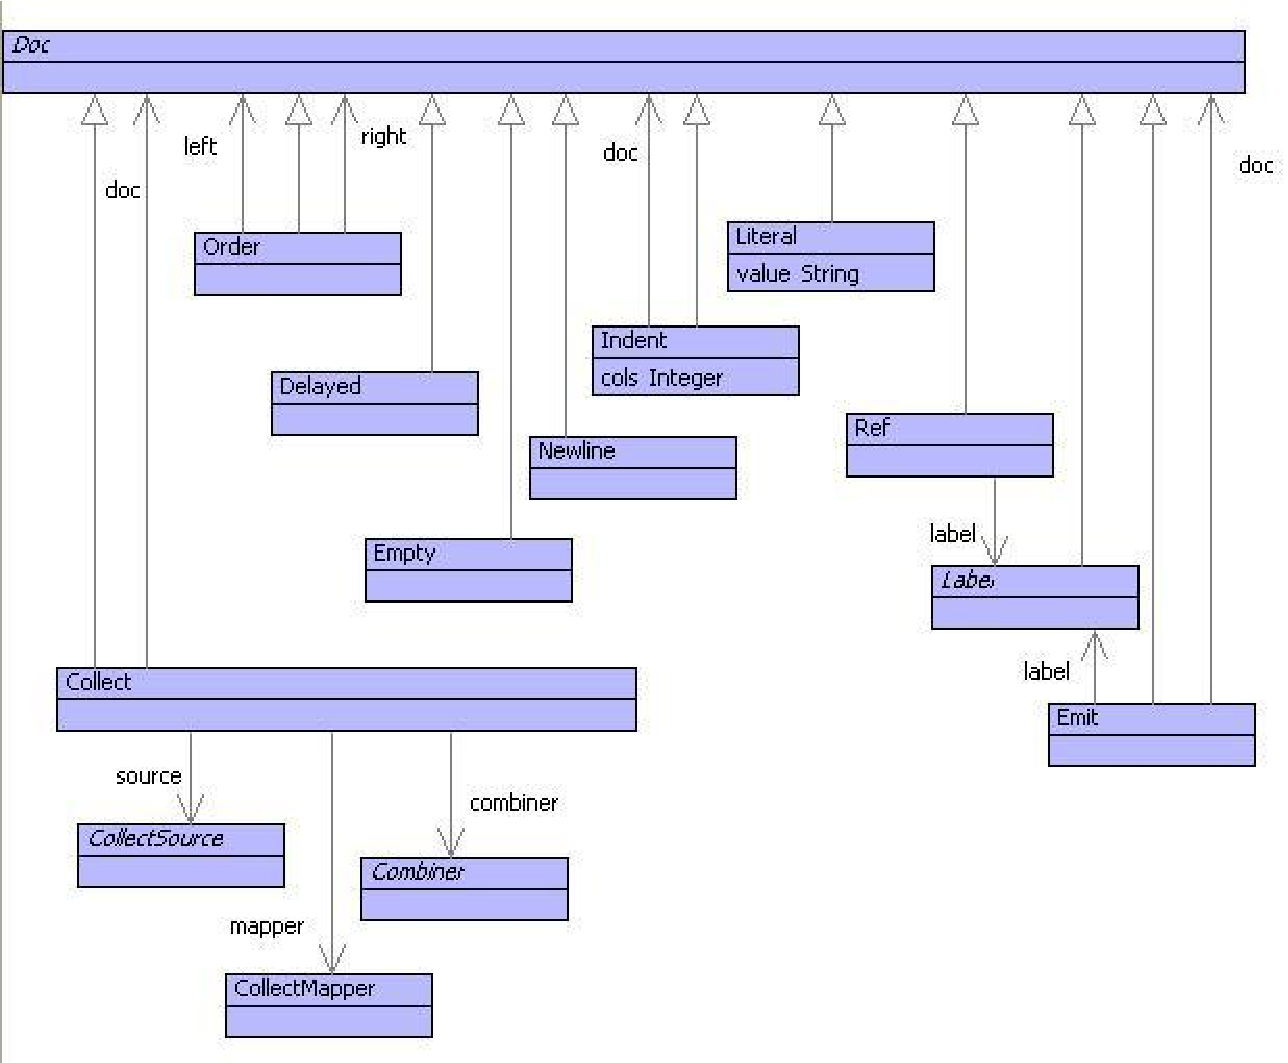
\includegraphics[width=12cm]{LanguageEngineering/DocComposition/Images/Doc}

\caption{Document Model\label{fig:Document-Model}}

\end{center}
\end{figure}


Once patterns have matched a collection of elements, document templates
are produced in the context of the matched environment. The document
model is shown in figure \ref{fig:Document-Model}. The model is used
in three ways: to represent document patterns in rules; to represent
document templates; to represent document displays. The difference
between these three uses is: patterns may contain delayed expressions;
templates may contain unresolved labels; document displays contain
no unresolved labels and no delayed expressions.

The classes in the model match the constructs in the language examples
from the previous section. The following classes are worth noting:
the source, mapper and combiner of a collect are classes that are
specialized in specific ways for different kinds of builtin collection
operations; Label is a class that is either specialized as a delayed
label or a literal label.

Delayed document components are used to allow arbitrary expressions
to be embedded. The expressions are to be evaluated when the document
is created in the context of the environment produced by successful
pattern matching. When the delayed document is created, the expression
is turned into an operation whose arguments correspond to the variable
names used in the expression. Delayed components include: source,
mapper and combiner of a collect; a delayed document; and a delayed
label.

The grammar for documents is shown below:

\begin{lstlisting}
@Grammar extends OCL::OCL.grammar
  Doc(FV) ::= d = AtomicDoc^(FV) DocTail^(FV,d).
  AtomicDoc(FV) ::= 
    Build^(FV) 
  | Delayed^(FV) 
  | Emit^(FV) 
  | Empty 
  | Newline 
  | Ref^(FV) 
  | Literal 
  | Indent^(FV) 
  | Label^(FV).
  DocTail(FV,d1) ::= 
    '+' d2 = Doc^(FV) { Order(d1,d2) } 
  | { d1 }.
  Build(FV) ::= 
    '{' s = Source^(FV) 
        m = Map^(FV) 
        c = Combiner d = Doc^(FV) 
    '}' {
       Collect(s,m,c,d) 
  }.
  Source(FV) ::= 
    LabelSource^(FV) 
  | DelayedSource^(FV).
  LabelSource(FV) ::= '[' e = Exp ']' op = DocOp^(FV,e) { 
    DelayedLabelSource(op) 
  }.
  Map(FV) ::= 
    '<' e = DelayedExp '>' op = DocOp^(FV,e) { 
       DelayedMapper(op) } 
  | 'id' { IdMap() }.
  DelayedSource(FV) ::= '<' e = Exp '>' op = DocOp^(FV,e) { 
    DelayedSource(op) 
  }.
  Combiner ::= 
   'nl' { CombineWithNewlines() } 
  | 'ignore' { Ignore() }.
  Label(FV) ::= '[' e = Exp ']' op = DocOp^(FV,e) { 
    DelayedLabel(op) 
  }.
  Delayed(FV) ::= '<' e = Exp '>' op = DocOp^(FV,e) { 
    Delayed(op)  
  }.
  Emit(FV) ::= 'emit' l = Label^(FV) d = Doc^(FV) { 
    Emit(l,d) 
  }.
  Empty ::= 'empty' { Empty() }.
  Newline ::= 'nl' { Newline() }.
  Ref(FV) ::= '!' l = Label^(FV) { Ref(l) }.
  Literal ::= s = Str { Literal(s) }.
  Indent(FV) ::= '->' '[' d = Doc^(FV) ']' { 
    Indent(2,d) 
  }.
  DocOp(FV,e) ::= { DocOp(FV,e) }.
end 
\end{lstlisting}The document grammar extends the OCL grammar in order to refer to
the Exp grammar rule for delayed document components. Many of the
grammar clauses for Doc are parameterized with respect to a set of
free variables. This feature allows delayed expressions to be transformed
into operations where the arguments of the operation are the intersection
of the free variables referenced in the expression and those bound
in the current pattern environment. For example, the rule:

\begin{lstlisting}
@Rule Class[name=n] -> "class " + <toUpper(n)> end
\end{lstlisting}contains a delayed expression: toUpper(n). The delayed expression
contains two free variables: toUpper and n. However, when the rule
fires, only one of the free variables (n) will be bound in the pattern
matching environment. The delayed expression is translated by the
parser into an operation:

\begin{lstlisting}
@Operation(n) toUpper(n) end
\end{lstlisting}where the arguments (n) are calculated as the intersection of the
free variables in the body \{toUpper,n\} and the variables bound by
the pattern \{n\}. Patterns implement an operation FV that calculates
the set of variables bound by the pattern; this set is supplied to
the Doc clauses. The set FV is ultimately used in the clause DocOp
that creates an instance of the class DocOp. A DocOp is just like
a normal operation except that its arguments are calculated by taking
the intersection of the FV and and free variables of its body.

The rest of the Doc grammar should be self explanatory. Note that
some classes are used that are not shown in figure \ref{fig:Document-Model}.
These are sub-classes of Label and collection classes; they capture
various special cases and associate them with special purpose syntax.


\subsection{Rules and Rule Bases}

%
\begin{figure}
\begin{center}

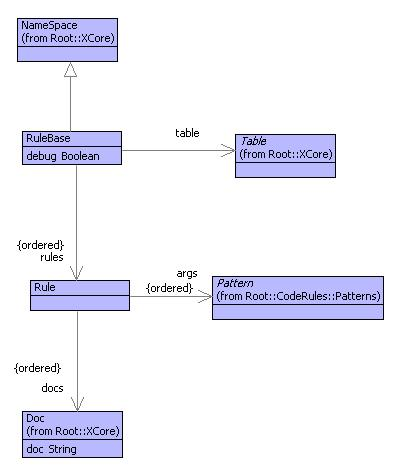
\includegraphics[width=12cm]{LanguageEngineering/DocComposition/Images/Rule}

\caption{Rule Model\label{fig:Rule-Model}}

\end{center}
\end{figure}


Figure \ref{fig:Rule-Model} shows the model of rules and rule bases.
A rule consists of a sequence of patterns and a sequence of documents.
A rule base is a sequence of rules that will be tried in turn when
the rule base is supplied with elements. A rule base has a table that
is used to hold associations between labels and documents when rules
are fired. On the resolution pass, labels are replaced with their
documents from the table. The table also allows particular documents
to be indexed by their name; for example only part of a document in
a large model can be re-generated.

The rest of this section describes how rules are fired and then the
resulting document is produced by resolving labels. Argument elements
are supplied to a rule base via the operation apply defined below. 

Each rule is applied to the args in turn until one is enabled by returning
a non-null environment. When this occurs the rule is fired, supplying
the environment to the rule. Notice that the environment is extended
with a binding for 'map' which allows the document to call the rule-base
again:

\begin{lstlisting}
context RuleBase
  @Operation apply(args)
    let done = false;
        result = null
    in @For rule in R when not done do
         let env = rule.match(args,Seq{})
         in if env <> null
            then
              let env = env->bind("map",
                   @Operation(.args)
                     self.apply(args)
                   end)
              in done := true; 
                 result := rule.fire(env,table)
              end
            end 
         end 
       end;
       if not done
       then self.error(formats("No rule for (~{,~;~S~}~%",Seq{args}))
       else result
       end
    end
  end
\end{lstlisting}Rules are matched using the match operation defined below which, in
turn, calls the match operation for each of the patterns:

\begin{lstlisting}
context Rule
  @Operation match(values,env)
    if args->size = values->size
    then 
      @For arg,value in args,values do
        if env <> null
        then env := arg.match(value,env)
        end
      end;
      env
    else null
    end
  end
\end{lstlisting}
\subsection{Forcing Delayed Documents}

A rule is fired by forcing its documents. Forcing a document causes
all of the delayed expressions to be evaluated and all 'emit' documents
to update the rule-base table:

\begin{lstlisting}
context Rule
  @Operation fire(env,table)
    let result = null
    in @For doc in docs do
         result := doc.force(env,table)
       end;
       result
    end
  end
\end{lstlisting}Forcing a document achieves two tasks:

\begin{itemize}
\item Components of a document may be delayed expressions that evaluate
to produce documents. These include expressions in < .. > and within
the {[} ... ] part of emit and label references. Forcing a document
evaluates the delayed expressions and returns the original document
with the delayed expressions replaced with the results.
\item Components of a document may be 'emit'-ed. Forcing a document updates
the document table with associations between the emit-label and the
emit-document (after delayed expressions have been evaluated).
\end{itemize}
Each document class defines a force operation that expects an environment
and a table. The environment is produces by the pattern matching and
contains values for free variables referenced in the delayed expressions.
The table is used to associate labels and documents produced by 'emit'.
Many of the force operations just force the sub-components, for example:

\begin{lstlisting}
context Collect
  @Operation force(env,table)
    // Just return the collect with the
    // components forced...
    Collect(
      source.force(env),
      mapper.force(env),
      combiner,
      doc.force(env,table))
  end
\end{lstlisting}Delayed expressions are implemented by associating documents with
operations. The arguments of the operation define the free variables
that must be supplied by the pattern matching environment. Components
with delayed expressions are implemented in the same way. Here is
the implementation of force for a delayed expression that occurs in
source code as <...>:

\begin{lstlisting}
context Delayed
  @Operation force(env,table)
    // Get the bindings from the environment that provide values
    // for the parameter names of the operation...
    let args = operation.paramNames()
                 ->collect(name | 
                    env->lookup(name.toString())) then
        // Force the delayed expression by supplying the argument
        // values...
        value = operation.invoke(self,args)
    in // Coerce the return value to be a document...
       @TypeCase(value)
         Doc do
           value
         end
         else Literal(value.toString())
       end
    end
  end
\end{lstlisting}Finally, an emit document updates the table:

\begin{lstlisting}
context Emit
  @Operation force(env,table)
        // Force the label...
    let label = label.force(env) then
        name = label.label();
        // Force the body...
        doc = doc.force(env,table)
    in // Extend the table with an entry for the label...
       if table.hasKey(name)
       then table.put(name,table.get(name) + Seq{doc})
       else table.put(name,Seq{doc})
       end;
       doc
    end
  end
\end{lstlisting}
\subsection{Displaying Documents}

Once rules have been fired and all documents have been forced, the
result is a table that associates labels with document templates.
A document template may contain label references; it is translated
to a document by replacing all the references. This is done using
the display operation of the rule base as shown below:

\begin{lstlisting}
@Operation display(label:String)
  // Display the document with the given label...
  if table.hasKey(label)
  then 
    // Use a string output buffer because there may be
    // lots of output...
    let buffer = Buffer(1000,true)
    in table.get(label)->at(0).display(0,table,buffer);
       buffer.toString()
    end
  else self.error("No label in table: " + label)
  end
end
\end{lstlisting}Each of the document classes defined an operation called display that
takes three arguments: the current level of indentation; the table
associating labels with document templates and an output buffer. Each
of the document classes implements the display operation differently.
The rest of this section describes how the documents are displayed.

The Collect class expects the collect source to produce a sequence
of documents, each of which is mapped and then combined to produce
a final single document that is displayed:

\begin{lstlisting}
@Operation display(indent,table,buffer)
  source.elements(table)->iterate(element doc = doc | 
    combiner.combine(doc,mapper.map(element)))
  .display(indent,table,buffer)
end
\end{lstlisting}A label reference requires that the label name is a key in the table.
The table should associate a collection of documents with the label
name; labels are used to reference the first element (collection documents
are used to combine multiple document entries in the table):

\begin{lstlisting}
@Operation display(indent,table,buffer)
  if table.hasKey(label)
  then table.get(label)->at(0).display(indent,table,buffer)
  else self.error("Label: cannot find label " + label)
  end
end
\end{lstlisting}A NewLine causes a new-line character to be added to the output buffer.
After each new-line, the current level of indentation is achieved
by adding the appropriate number of spaces:

\begin{lstlisting}
@Operation display(indent,table,buffer)
  buffer.add("\n"->at(0));
  buffer.append(formats("~V",Seq{indent}))
end
\end{lstlisting}Ordered documents just display the first and then the second:

\begin{lstlisting}
@Operation display(indent,table,buffer)
  left.display(indent,table,buffer);
  right.display(indent,table,buffer)
end
\end{lstlisting}
